\section{Requisitos}

    Esta seção trará todos os requisitos e restrições que os projetos e seus respectivos relatórios devem atender para estarem aptos ao lançamento, sendo que o descumprimento de qualquer requisito acarretará na desqualificação da equipe.
    
    Os relatórios produzidos devem explicitar claramente o cumprimento de todos os requisitos aqui presentes. Abaixo seguem os requisitos correspondentes a cada modalidade de competição.

    \subsection{PseudoSat}    
    A seguir estão listados os requisitos para missões na modalidade PseudoSat.

    \begin{definition}[1]
    Os SmallSats deverão ter massa máxima (invólucro + experimento) de 30g. Enquanto isso, os BigSats deverão ter massa máxima de 120g.
    \end{definition}
    
    \begin{definition}[2]
    O experimento planejado para o SmallSat deve possuir um volume máximo de 50 x 50 x 50 mm, que será contido no seguinte recipiente:
    
    \centering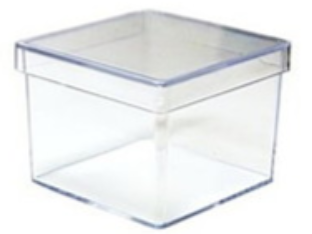
\includegraphics[width=0.4\textwidth]{Figures/smallsat.png}
    
    \justifying Já o experimento planejado para o BigSat deve possuir um volume máximo de 80 x 80 x 50 mm, que será contido no seguinte recipiente:
    
    \centering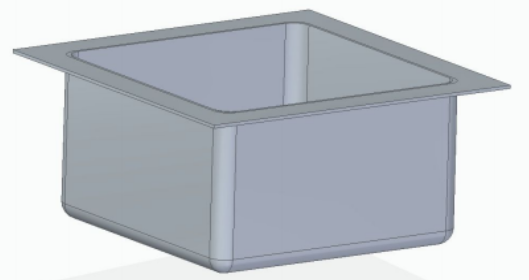
\includegraphics[width=0.5\textwidth]{Figures/bigsat.png}
    
    \justifying Ambos os recipientes serão fornecidos pelo grupo Zenith às equipes classificadas que efetivarem sua participação na Fase 2. Estender verticalmente acima do invólucro é permitido, desde que não afete o próprio experimento ou os demais presentes na sonda.
    \end{definition}
    
    \begin{definition}[3]
    O experimento deve possuir um sistema de fixação robusto previamente planejado pela equipe, que suporte fortes impactos e variações abruptas de velocidade, além de impedir possíveis vazamentos ou escape de partes do experimento. Os SATs que forem considerados mal fixados e que possam causar riscos para a sonda-mãe, ou para os demais experimentos, poderão ser desclassificados mesmo após a chegada do experimento para lançamento.
    \end{definition}
    
    \begin{definition}[4]
    Os PseudoSats deverão conter a identificação adesivada, com o nome da equipe e da escola participante.
    \end{definition}
    
    \begin{definition}[5]
    Por questões éticas, não será permitido animais nem embriões de quaisquer espécies nos PseudoSats. Plantas, bactérias e fungos serão permitidos mediante aprovação da comissão avaliadora com base na Proposta Experimental.
    
    *Seres patogênicos para animais e plantas serão proibidos. Animais cordados e embriões são proibidos. Culturas celulares, permitidas. Ovos de artrópodes são permitidos. Exceções mediante aprovação.
    \end{definition}
    
    \begin{definition}[6]
    O uso de radiofrequências para comunicação ou transmissão de dados deve ser feito em conjunto com um radioamador autorizado, providenciado pelo grupo, dentro dos limites impostos pela ANATEL. As frequências e protocolos de comunicação devem ser informados.
    
    Sistemas de comunicação conflitantes entre participantes serão informados, caso em que será discutido um plano de frequências e timeslots a serem obedecidos pelas equipes.
    \end{definition}
    
    \begin{definition}[7]
    Não serão permitidos materiais explosivos, detonadores e quaisquer substâncias pirotécnicas ou inflamáveis. Baterias e substâncias químicas voláteis serão permitidas perante aprovação pela comissão avaliadora com base na Proposta Experimental.
    \end{definition}
    
    \begin{definition}[8]
    Experimentos que afetem as condições ambientais da sonda, ou de alguma forma prejudicarem os dados dos sensores da sonda, não serão permitidos.
    
    Exemplo: Um projeto que emita luz excessiva, campo magnético intenso ou produza calor exagerado.
    \end{definition}
    
    \begin{definition}[9]
    Eventuais baterias deverão estar em locais de fácil acesso caso haja necessidade de troca e/ou recarga. Para a recarga, deve haver um conector fornecido pelo proprietário do experimento,  algum tipo de indicador de carregamento e indicador de carga completa, de forma que se possa identificar o estado das baterias no experimento.
    
    Quanto à troca, o conector para as baterias deve ser simples e não deve exigir conhecimentos específicos por parte dos membros do Zenith. Todos os procedimentos necessários ao manuseio do sistema de alimentação do experimento devem estar descritos na Ficha de Dados.
    \end{definition}
    
    \begin{definition}[10]
    Caso hajam sistemas eletrônicos nos experimentos, como microcontroladores e computadores embarcados, o acionamento deverá ser feito por \textbf{apenas} uma chave identificada com indicação de ligado/desligado. Membros do Zenith ligarão o experimento em até 15 minutos antes do lançamento, e desligarão o SAT assim que a sonda for resgatada.
    \end{definition}
    
    \begin{definition}[11]
    Experimentos que contenham algum tipo de líquido deverão especificar como será o armazenamento do mesmo e, após análise, poderão ser recusados caso exista a possibilidade de ocorrerem vazamentos.
    \end{definition}
    

    \subsection{FullSat}
    A seguir estão listados os requisitos para missões na modalidade FullSat.

    \begin{definition}[1]
    Os FullSats devem atender ao form factor de CanSat (6,5 cm de diâmetro e 10 cm de altura) ou do CubeSat 1U (100 x 100 x 100 mm), conforme especificado na Proposta Experimental.
    \end{definition}

    \begin{definition}[2]
    A massa máxima permitida para o CanSat é 400g, e para o CubeSat 500g.
    \end{definition}

    \begin{definition}[3]
    O satélite deve ser capaz de operar a 35km de altitude, possuindo isolamento térmico para componentes sensíveis à temperatura.
    \end{definition}

    \begin{definition}[4]
    O satélite deve ser capaz de coletar e armazenar dados de telemetria durante o voo, especificamente:
    \begin{enumerate}
        \item Status da bateria;
        \item Pressão;
        \item Temperatura;
        \item Atitude e acelerômetro;
        \item Demais itens pertinentes à missão.
    \end{enumerate}
    \end{definition}

    \begin{definition}[7]
    Equipes que buscam realizar transmissão de dados via rádio entre o satélite desenvolvido e o solo devem providenciar um radioamador responsável e garantir que suas transmissões sigam diretrizes estabelecidas pela Anatel.
    
    O uso de comunicação via rádio deve ser indicada ao Zenith, junto às frequências e protocolos utilizados. Sistemas de comunicação conflitantes entre participantes serão informados, caso em que será discutido um plano de frequências e timeslots a serem obedecidos pelas equipes.
    \end{definition}

    \begin{definition}[5]
    Deve-se apresentar um sistema mecânico robusto e bem montado, resistente a impactos e vibrações, indicando o cumprimento do requisito por meio de simulações e ensaios estruturais.
    \end{definition}
    
    \begin{definition}[6]
    A base do satélite deve ser equivalente aos projetos de tampa trazidos no apêndice, para fixação na sonda durante o lançamento.
    \end{definition}

    \begin{definition}[7]
    O acionamento do satélite deverá ocorrer \textbf{apenas} por uma chave identificada com indicação de ligado/desligado. Membros do Zenith ligarão o experimento em até 15 minutos antes do lançamento, e desligarão o satélite assim que a sonda for resgatada.
    \end{definition}

    \begin{definition}[8]
    Experimentos que afetem as condições ambientais da sonda, ou de alguma forma prejudicarem os dados dos sensores da sonda, não serão permitidos.
    
    Exemplo: Um projeto que emita luz excessiva, campo magnético intenso ou produza calor exagerado.
    \end{definition}